\documentclass[landscape,final,a0paper]{baposter}


\tracingstats=2

\usepackage{calc}
\usepackage{graphicx}
\usepackage{amsmath}
\usepackage{amssymb}
\usepackage{relsize}
\usepackage{multirow}
\usepackage{bm}

\usepackage{graphicx}
\usepackage{multicol}

\usepackage{pgfbaselayers}
\pgfdeclarelayer{background}
\pgfdeclarelayer{foreground}
\pgfsetlayers{background,main,foreground}

\usepackage{times}
\usepackage{helvet}
\usepackage{palatino}
\usepackage[utf8x]{inputenc}
\usepackage{amssymb, upgreek}

\usepackage{color}
\definecolor{keywordcolor}{rgb}{0.7, 0.1, 0.1}   % red
\definecolor{commentcolor}{rgb}{0.4, 0.4, 0.4}   % grey
\definecolor{symbolcolor}{rgb}{0.0, 0.1, 0.6}    % blue
\definecolor{sortcolor}{rgb}{0.1, 0.5, 0.1}      % green
\definecolor{errorcolor}{rgb}{1, 0, 0}           % bright red
\definecolor{stringcolor}{rgb}{0.5, 0.3, 0.2}    % brown

\usepackage{listings}
\def\lstlanguagefiles{lstlean.tex}
\lstset{language=lean}

\usepackage[hyphens]{url}

\DeclareUrlCommand\url{\color{magenta}\def\UrlLeft{http://}\urlstyle{tt}}

\newcommand{\captionfont}{\footnotesize}

\selectcolormodel{cmyk}

%\graphicspath{{images/}}

%%%%%%%%%%%%%%%%%%%%%%%%%%%%%%%%%%%%%%%%%%%%%%%%%%%%%%%%%%%%%%%%%%%%%%%%%%%%%%%%
%%%% Some math symbols used in the text
%%%%%%%%%%%%%%%%%%%%%%%%%%%%%%%%%%%%%%%%%%%%%%%%%%%%%%%%%%%%%%%%%%%%%%%%%%%%%%%%
% Format 

\renewcommand{\Pr}{\mbox{P}}
\newcommand{\e}{\mbox{e}}
\newcommand{\dx}{\,\mbox{d}x}

%%%%%%%%%%%%%%%%%%%%%%%%%%%%%%%%%%%%%%%%%%%%%%%%%%%%%%%%%%%%%%%%%%%%%%%%%%%%%%%%
% Multicol Settings
%%%%%%%%%%%%%%%%%%%%%%%%%%%%%%%%%%%%%%%%%%%%%%%%%%%%%%%%%%%%%%%%%%%%%%%%%%%%%%%%
\setlength{\columnsep}{0.7em}
\setlength{\columnseprule}{0mm}


%%%%%%%%%%%%%%%%%%%%%%%%%%%%%%%%%%%%%%%%%%%%%%%%%%%%%%%%%%%%%%%%%%%%%%%%%%%%%%%%
% Save space in lists. Use this after the opening of the list
%%%%%%%%%%%%%%%%%%%%%%%%%%%%%%%%%%%%%%%%%%%%%%%%%%%%%%%%%%%%%%%%%%%%%%%%%%%%%%%%
\newcommand{\compresslist}{%
\setlength{\itemsep}{1pt}%
\setlength{\parskip}{0pt}%
\setlength{\parsep}{0pt}%
}


%%%%%%%%%%%%%%%%%%%%%%%%%%%%%%%%%%%%%%%%%%%%%%%%%%%%%%%%%%%%%%%%%%%%%%%%%%%%%%
%%% Begin of Document
%%%%%%%%%%%%%%%%%%%%%%%%%%%%%%%%%%%%%%%%%%%%%%%%%%%%%%%%%%%%%%%%%%%%%%%%%%%%%%

\begin{document}

%%%%%%%%%%%%%%%%%%%%%%%%%%%%%%%%%%%%%%%%%%%%%%%%%%%%%%%%%%%%%%%%%%%%%%%%%%%%%%
%%% Here starts the poster
%%%---------------------------------------------------------------------------
%%% Format it to your taste with the options
%%%%%%%%%%%%%%%%%%%%%%%%%%%%%%%%%%%%%%%%%%%%%%%%%%%%%%%%%%%%%%%%%%%%%%%%%%%%%%
% Define some colors
\definecolor{silver}{cmyk}{0,0,0,0.3}
\definecolor{yellow}{cmyk}{0,0,0.9,0.0}
\definecolor{reddishyellow}{cmyk}{0,0.22,1.0,0.0}
\definecolor{black}{cmyk}{0,0,0.0,1.0}
\definecolor{darkYellow}{cmyk}{0,0,1.0,0.5}
\definecolor{darkSilver}{cmyk}{0,0,0,0.1}
\definecolor{lightyellow}{cmyk}{0,0,0.3,0.0}
\definecolor{lighteryellow}{cmyk}{0,0,0.1,0.0}
\definecolor{lighteryellow}{cmyk}{0,0,0.1,0.0}
\definecolor{lightestyellow}{cmyk}{0,0,0.05,0.0}
\definecolor{cyan}{cmyk}{1,0,0,0}
\definecolor{lightcyan}{cmyk}{0.5,0,0,0}
\definecolor{pastelcyan}{cmyk}{0.25,0,0,0}
\definecolor{magenta}{cmyk}{0,1,0,0}
\definecolor{yellow}{cmyk}{0,0,1,0}
\definecolor{lightyellow}{cmyk}{0,0,0.5,0}
\definecolor{pastelyellow}{cmyk}{0,0,0.25,0}
\definecolor{black}{cmyk}{0,0,0,1}
\definecolor{darkgray}{cmyk}{0,0,0,0.75}
\definecolor{gray}{cmyk}{0,0,0,0.5}
\definecolor{lightgray}{cmyk}{0,0,0,0.25}
\definecolor{white}{cmyk}{0,0,0,0}
\definecolor{red}{cmyk}{0,1,1,0}
\definecolor{orange}{cmyk}{0,0.5,1,0}
\definecolor{scarlet}{cmyk}{0,1,0.5,0}
\definecolor{brown}{cmyk}{0.5,0.75,1,0}
\definecolor{camel}{cmyk}{0.25,0.375,0.5,0}
\definecolor{cream}{cmyk}{0,0.2,0.3,0}
\definecolor{green}{cmyk}{1,0,1,0}
\definecolor{lightgreen}{cmyk}{0.5,0,0.5,0}
\definecolor{pastelgreen}{cmyk}{0.25,0,0.25,0}
\definecolor{mossgreen}{cmyk}{0.64,0.4,1,0}
\definecolor{yellowgreen}{cmyk}{0.5,0,1,0}
\definecolor{skyblue}{cmyk}{0.4,0.16,0,0}
\definecolor{royal}{cmyk}{1.0,0.5,0,0}
\definecolor{navyblue}{cmyk}{0.9,0.75,0.5,0}
\definecolor{lightnavy}{cmyk}{0.4,0.3,0.2,0}
\definecolor{blue}{cmyk}{1,1,0,0}
\definecolor{lightblue}{cmyk}{0.5,0.5,0,0}
\definecolor{pastelblue}{cmyk}{0.25,0.25,0,0}
\definecolor{lightpastelblue}{cmyk}{0.15,0.15,0,0}
\definecolor{lightestpastelblue}{cmyk}{0.05,0.05,0,0}
\definecolor{lavender}{cmyk}{0.25,0.25,0,0}
\definecolor{violet}{cmyk}{0.75,1,0.25,0}
\definecolor{purple}{cmyk}{0.5,1,0.5,0}
\definecolor{lightpurple}{cmyk}{0.25,0.5,0.25,0}
\definecolor{pink}{cmyk}{0,0.5,0,0}


%%

\typeout{Poster Starts}
%\background{
  %\begin{tikzpicture}[remember picture,overlay]%
  %  \draw (current page.north west)+(-2em,-2em) node[anchor=north west] %{\hspace{-2em}\includegraphics[height=1.1\textheight]{silhouettes_background}};
 % \end{tikzpicture}%
%}




\newlength{\leftimgwidth}
\begin{poster}%
  % Poster Options, such as colours etc
  {
  % Show grid to help with alignment
  grid=false,
 % Column spacing
  colspacing=0.5em,
 % Color style
 % bgColorOne=pastelblue,
 %bgColorTwo=lightpastelblue,
  bgColorOne=white,
  bgColorTwo=white,
  borderColor=navyblue,
  headerColorOne=lightnavy,
  headerColorTwo=purple,
  headerFontColor=black,
 % boxColorOne=lightpastelblue,
 % boxColorTwo=lightestpastelblue,
 boxColorOne=white,
 boxColorTwo=white,
 % Format of textbox
  textborder=roundedleft,
% textborder=rectangle,
% Format of text header
  eyecatcher=false,
  headerborder=open,
  headerheight=0.08\textheight,
  headershape=roundedright,
  headershade=plain,
  headerfont=\Large\textsf, %Sans Serif
  boxshade=plain,
%  background=shade-tb,
 % background=plain,
  background=none,
  linewidth=2pt
  }
  % Eye Catcher
  {} % select eyecatcher=false above if not required. If no eye catcher is present, the title is left aligned.
  % Title
  {\sf %Sans Serif
  %\bf% Serif
  \vspace*{5mm}
  \hspace*{2mm} The Formalisation and Applications of the Stone-Weierstrass Theorem}
  % Authors
  {\linebreak
  \hspace*{4.5mm} Kexing Ying
  }
  % University logo
  { % The makebox allows the title to flow into the logo
    \makebox[8em][r]{%
        \begin{minipage}{16em}
				\hfill 
\includegraphics[height=3em]{imperial.pdf}
				\end{minipage}
      
    }
  }

  \tikzstyle{light shaded}=[top color=baposterBGtwo!30!white,bottom color=baposterBGone!30!white,shading=axis,shading angle=30]

  % Width of left inset image
     \setlength{\leftimgwidth}{0.78em+8.0em}

%%%%%%%%%%%%%%%%%%%%%%%%%%%%%%%%%%%%%%%%%%%%%%%%%%%%%%%%%%%%%%%%%%%%%%%%%%%%%%
%%% Now define the boxes that make up the poster
%%%---------------------------------------------------------------------------
%%% Each box has a name and can be placed absolutely or relatively.
%%% The only inconvenience is that you can only specify a relative position 
%%% towards an already declared box. So if you have a box attached to the 
%%% bottom, one to the top and a third one which should be in between, you 
%%% have to specify the top and bottom boxes before you specify the middle 
%%% box.
%%%%%%%%%%%%%%%%%%%%%%%%%%%%%%%%%%%%%%%%%%%%%%%%%%%%%%%%%%%%%%%%%%%%%%%%%%%%%%
    %
    % A coloured circle useful as a bullet with an adjustably strong filling
\newcommand{\colouredcircle}[1]{%
      \tikz{\useasboundingbox (-0.2em,-0.32em) rectangle(0.2em,0.32em); \draw[draw=black,fill=baposterBGone!80!black!#1!white,line width=0.03em] (0,0) circle(0.18em);}}

  \headerbox{The Stone-Weierstrass Theorem}{name=stone,column=0,span=1, row=0}{
\textit{The Stone-Weierstrass theorem} states that, given an unital subalgebra of $M$, $M_0$ that is 
closed under lattice operations and separates points, $\bar{M_0} = M$, and we say $M_0$ is dense in $M$ \cite{gaddy}.

This theorem is important as not only does it offer a strong result regarding function spaces, it also offers insight into interpolation as it demonstrates which set of functions can act as basis for a particular function space. 
 }

%%%%%%%%%%%%%%%%%%%%%%%%%%%%%%%%%%%%%%%%%%%%%%%%%%%%%%%%%%%%%%%%%%%%%%%%%%%%%%
  \headerbox{Variables and Definitions}{name=notations,column=0,below=stone}{
%%%%%%%%%%%%%%%%%%%%%%%%%%%%%%%%%%%%%%%%%%%%%%%%%%%%%%%%%%%%%%%%%%%%%%%%%%%%%%
Throughout this poster, we will let $X$ be a compact metric space, $M$ to be the set of all 
bounded and continuous functions from $X$ to $\mathbb{R}$, $M_0$ a subset of $M$ and 
$\bar{M_0}$ the closure of $M_0$ \textit{under uniform convergence to the limit}.

We say $M_0$ \textit{separates points} if and only if for all distinct $x, y \in X$, there 
exists some $f \in M_0$ such that $f(x) \neq f(y)$.

Given $x, y \in X$, the boundary points of $M_0$ is defined to be $\{(f(x), f(y)) \mid f \in M_0 \}$.

  \vspace{0.3em}
  }

%%%%%%%%%%%%%%%%%%%%%%%%%%%%%%%%%%%%%%%%%%%%%%%%%%%%%%%%%%%%%%%%%%%%%%%%%%%%%%
  \headerbox{Lattice Operations}{name=lattice,column=0,below=notations}{
%%%%%%%%%%%%%%%%%%%%%%%%%%%%%%%%%%%%%%%%%%%%%%%%%%%%%%%%%%%%%%%%%%%%%%%%%%%%%%
We define two lattice operations \(\vee, \wedge : (X \to \mathbb{R})^2\to (X \to \mathbb{R}) \) 
such that, for all \(f, g : X \to \mathbb{R}\), where \(f, g\) are bounded continuous functions 
$$
f \vee g = \max\{f, g\}; \hspace{2mm} f \wedge g = \min \{f, g\}.
$$

  \vspace{0.3em}
  }

%%%%%%%%%%%%%%%%%%%%%%%%%%%%%%%%%%%%%%%%%%%%%%%%%%%%%%%%%%%%%%%%%%%%%%%%%%%%%%
  \headerbox{$R$-algebra and Subalgebra}{name=algebra,column=0,below=lattice}{
%%%%%%%%%%%%%%%%%%%%%%%%%%%%%%%%%%%%%%%%%%%%%%%%%%%%%%%%%%%%%%%%%%%%%%%%%%%%%%
An \textit{$R$-algebra} is a mathematical object consisting of a commutative ring $R$ and a 
semi-ring $A$ such that there exists scalar multiplication \(\cdot : R \times A \to A\) 
and a homomorphism from $R$ to $A$, \(\phi : R \to A\) such that 
$$
r \cdot a = \phi(r) \times a,
$$
and 
$$
\phi(r) \times a = a \times \phi(r),
$$
are satisfied for all $r \in R$ and $a \in A$ \cite{lau}.

A \textit{unital subalgebra} $S$ of an $R$-algebra $A$ is a subset of $A$ that's closed under the induced operations 
carried from $A$ and contains 1 \cite{lau}. 

\vspace{2.6mm}
It was shown that both $M$ and $\mathbb{R}^2$ form a $R$-algebra over $\mathbb{R}$ (see: \url{bit.ly/3eL7LEC}).

  \vspace{0.3em}
  }

%%%%%%%%%%%%%%%%%%%%%%%%%%%%%%%%%%%%%%%%%%%%%%%%%%%%%%%%%%%%%%%%%%%%%%%%%%%%%%
  \headerbox{Application: Weierstrass Theorem}{name=approx,column=1,span=1,row=0}{
	
The Stone-Weierstrass theorem is a generalisation of the Weierstrass approximation theorem which states that any continuous functions on 
a closed interval can be uniformly approximated by a polynomial. This can be deduced straightaway by the Stone-Weierstrass theorem.

\vspace{2mm}
Consider the Taylor polynomial $P_n(x)$ of $s(x)= \sqrt{1- x}$ for $x \in [-1, 1]$. Using analysis, we can show that $P_n \to s$ uniformly, 
and thus, $P_n(1-x^2) \to s(1-x^2)= \left| x \right|$ uniformly for $x \in [-1, 1]$. Now, as 
$$f \vee g = \max \{f, g\} = \frac{1}{2}(f + g + \left| f - g \right|);$$
$$f \wedge g = \min \{f, g\} = \frac{1}{2}(f + g - \left| f - g \right|),$$
we see that if $\bar{\mathcal{P}}$ is the closure of the set of polynomials under uniform convergence to the limit, $\bar{\mathcal{P}}$ would 
also be closed under the lattice operations. Thus, as $\bar{\mathcal{P}}$ form an unital subalgebra of all real to real functions, (as its closed under 
addition and multiplication), and as $\bar{\mathcal{P}}$ separates points trivially, $\bar{\bar{\mathcal{P}}} = \bar{\mathcal{P}} = [-1, 1]^\mathbb{R}$ which can be trivially extended to any closed intervals as required.

\vspace{2mm}
However, this can also be proved by constructing the approximant directly. By using 
the weak law of large numbers, we can prove that the Bernstein polynomials can be used 
to find a sequence of polynomials that uniformly converges on any continuous function.
(A full proof was typed up and is presented here: \url{bit.ly/2Mz8ug8})
  \vspace{0.2em}
  }

 \headerbox{Application: Trig. Polynomials}{name=trig,column=1,span=1,below=approx}{
 
Another set of functions we might be interested in are the trigonometric polynomials $\mathcal{T}$ 
where trigonometric polynomials are functions of the form
\[f(x) = a_0 + \sum_{k = 1}^n a_k \cos(kx) + b_k \sin(kx); \hspace{1mm} a_i, b_i \in \mathbb{R}.\]

As the trigonometric polynomials $\mathcal{T}$ form an unital subalgebra of the
bounded continuous functions on \([-\pi, \pi]\) (by considering the identities 
of multiplication between trigonometric functions),
and by considering the Fourier series of $\left| x \right|$, by the same argument as presented above,
$\bar{\mathcal{T}}$ is closed under lattice operations and hence, by Stone-Weierstrass, 
$\bar{\bar{\mathcal{T}}} = \bar{\mathcal{T}} = [-\pi, \pi]^\mathbb{R}$

  \vspace{0.2em}
  }

 \headerbox{Further Discussion \& Interpolation}{name=inter,column=3,span=1,row=0}{
 While the Stone-Weierstrass theorem proved existence, and the Bernstein polynomials offerd us a method to find a polynomial arbitrarily close to any continuous function with respect to the uniform norm, it is not necessarily the best approximation.

\vspace{2mm}
Using some simple \textit{Python} scripts, we can easily see that for functions such as $x^2$, the Bernstein 
polynomials does not offer as much accuracy as just using $x^2$ as its own approximation.
\begin{center}
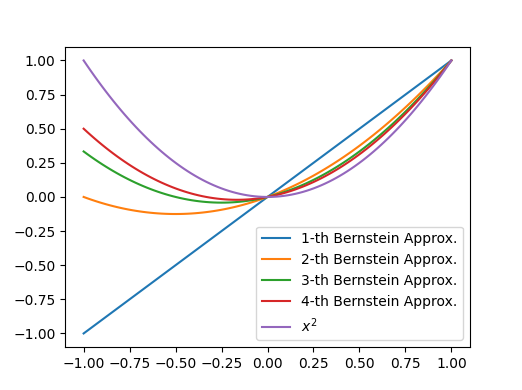
\includegraphics[scale = 0.515]{x_squared}
\end{center}
\vspace{-2mm}
Consider instead the interpolation theorem:

\textbf{Theorem.} Given $\{(x_0, y_0), \cdots, (x_n, y_n) \} \subseteq \mathbb{R}^2$, using Lagrange polynomials, we can construct polynomial that interpolates the set. \cite{humph}

\vspace{2mm}
So, if we let $f : [a, b] \to \mathbb{R}$ be a continuous function, we can approximate $f$ using the polynomial that interpolates the set of equidistant points from $a$ to $b$. By implementing this algorithm in Python, we find that for $n = 3$ for $f : [-1, 1] \to \mathbb{R}: x \mapsto x^2$, this method results in a polynomial approximation of $x^2$ (Very Good!). 

\vspace{2mm}
However, unlike the Bernstein polynomial method, this method does not guarantee that the uniform norm of the difference of the function and its approximation tends to zero as demonstrated by interpolating \textit{Runge's function} (it in fact tends to $+ \infty$). To mitigate this, one can instead use Spline interpolation however this results in an approximant that is a piecewise polynomial instead of just a polynomial.

  \vspace{0.2em}
  }  

 %%%%%%%%%%%%%%%%%%%%%%%%%%%%%%%%%%%%%%%%%%%%%%%%%%%%%%%%%%%%%%%%%%%%%%%%%%%%%
\headerbox{Outline and Formalisation}{name=form,column=2,span=1,row=0}{

\textit{The Stone-Weierstrass theorem} was proved and formalised using the 
\textit{Lean}, the source code of which can be found 
in my GitHub repository:\\ \url{github.com/JasonKYi/stone-weierstrass}. 

\vspace{2mm}
The theorem itself relies on two central lemmas:

{\bf Lemma 1.} For all $f \in M$, $f \in \bar{M_0}$ if and only if for all $x, y \in X$, $\epsilon > 0$, there 
exists $g \in M_0$ such that $\left| f(x) - g(x) \right| < \epsilon$ and $\left| f(y) - g(y) \right| < \epsilon$.

{\bf Lemma 2.} Given $S$, a subalgebra of $\mathbb{R}^2$, $S$ must be $\{(0,0)\}$, 
$\{(x, 0) \mid x \in \mathbb{R} \}$,
$\{(0. y) \mid y \in \mathbb{R} \}$, 
$\{(z, z) \mid z \in \mathbb{R} \}$, or
$\mathbb{R}^2$ itself.

\vspace{2mm}
\textit{Lemma 1} was formalised and is represented in Lean as 
$\tt{in\_closure₂\_iff\_dense\_at\_points}$ in $\tt{main.lean}$ by constructing
constructing mappings from $X$ to set of $X$ while considering the compactness of $X$;
while \textit{Lemma 2} was also formalised and is represented in Lean as $\tt{subalgebra\_of\_R2}$ and can be found in $\tt{ralgebra.lean}$ which proof involved evoking the law of the excluded middle on different propositions.
multiple times.

\vspace{2mm}
Now, let $M_0$, $M_1$ be closed subalgebras of $M$ under lattice operations,
then, by considering lemma 1, it was deduced $\bar{M_0} = \bar{M_1}$ if and only if at for all distinct $x$, $y$, $\bar{M_0}$ and $\bar{M_1}$ have the same boundary points. This was formalised in $\tt{eq\_iff\_boundary\_points\_eq}$ in $\tt{main.lean}$

\vspace{2mm}
Finally. by showing that the boundary points of $M_0$ form an unital subalgebra of $\mathbb{R}^2$, we see that the boundary points of  $\bar{M_0}$ must be $\mathbb{R^2}$ by lemma 2 and hence, as the boundary points of $M$ is $\mathbb{R}^2$ is $\mathbb{R}^2$, it follows $\bar{M_0} = M$. As required!

\vspace{2mm}
This was formalised in Lean in $\tt{main.lean}$ with the theorem statement being

\vspace{2mm}
\lstinline{theorem weierstrass_stone \{M₀' : subalgebra ℝ (X → ℝ)\} 
(hc   : closure₀ M₀'.carrier = M₀'.carrier)
(hsep : has_seperate_points M₀'.carrier) :
closure₂ M₀'.carrier = univ}


\vspace{0.2em}
  }
	
%%%%%%%%%%%%%%%%%%%%%%%%%%%%%%%%%%%%%%%%%%%%%%%%%%%%%%%%%%%%%%%%%%%%%%%%%%%%%%
  \headerbox{References}{name=references,column=2,span=2,below=form}{
    \smaller
    \vspace{-0.4em}
    \bibliographystyle{plain}
    \renewcommand{\section}[2]{\vskip 0.05em}
      \begin{thebibliography}{1}\itemsep=-0.01em
      \setlength{\baselineskip}{0.4em}
      \bibitem{stone}
        Stone, M.H.
        \newblock (1948) The Generalized Weierstrass Approximation Theorem.
        \newblock Mathematics Magazine 21, no. 5 : 237-54. 
      \bibitem{gaddy}
        Gaddy, P.
        \newblock The Stone-Weierstrass Theorem and its Applications to $L^2$ Spaces.
	  \bibitem{lau}
				Lau, K. and Kudryashov, Y.
				\newblock (2018) Algebra over Commutative Semiring (under category) [Online].
				\newblock Available at: \url{bit.ly/3gLIPyS}
				\newblock (Assessed: 02 June 2020)
	  \bibitem{humph}
	  	 Humpherys, J. and Jarvis, T. J.
	  	\newblock (2020) Foundations of Applied Mathematics Volume 2: Algorithms, Approximation, Optimization
	  	\newblock Society for Industrial and Applied Mathematics, pp. 418
      \end{thebibliography}
  }
%%%%%%%%%%%%%%%%%%%%%%%%%%%%%%%%%%%%%%%%%%%%%%%%%%%%%%%%%%%%%%%%%%%%%%%%%%%%%%
  
\end{poster}

\end{document}
